Throughout this course we were given the task of continuously improving and adding features to a legacy code base. The code base in question was an aging mini version of Twitter called \textit{Minitwit}. 

\section*{Technologies}

\subsection*{Refactoring}

Minitwit was originally written in Python 2 using Flask. The goal was to get the website running on a modern framework, this was done by firstly using the library 2to3, which converts python 2 code into python 3 code. Lastly to complete the refactoring we rewrote the code to run using the Django framework.

\subsection*{Containerized}

Containerized is a term in software development, which references the fact that you isolate part of your software into containers. To implement this technology we decided to use Docker. Using such technologies is beneficial when writing in teams, since you can keep all the moving parts isolated, thus solving the exponentially difficult problem of dependencies. By forcing everyone to use the dependencies within the container, this enables the container to be run on any computer/server having docker installed.
\\\\
We setup a total of 4 Docker containers each responsible for one specific task as seen below:


\begin{enumerate}
    \item Django server - one of the things we are hosting the ip
    \item Database - postgres container 
    \item Prometheus container, collecting data from Django container, how many requests monitoring
    \item Grafana visualization of performance i.e. monitoring
\end{enumerate}

\subsection*{Continuous Integration and Continuous Deployment}

DevOps is a development method where the time from the testing environment to production is rapidly shortened using automation to ensure high quality. Since we are using GitHub as our version control tool, we can use built in system for testing before deploying. GitHub has a built in CI/CD tool where you can build a pipeline of checks that have to be completed for the branches to be merged.

\subsection*{Cloud}

Since we are creating a web app, we need to host it somewhere, since we do not want our development computers to function as the server. By having a centralized structure, that is, a singular place for hosting, we only had to know one provider, and everyone could connect to it from anywhere. We used a Infrastructure-as-a-Service (IaaS) provider called Digital Ocean, due to them having a nice UX-design and allows for easy horizontal and vertical scaling.

\subsection*{Monitoring}

Monitoring is the act of getting information about the system. An important aspect of monitoring is choosing what to monitor, since it doesn't make sense to log and measure every part of the system, because this would take an unreasonable amount of space. Therefore you need to be selective with what metrics you monitor, to give only the insights you require. This can be anything from the technical aspect of uptime/availability, to more subjective things such as how the users rate your service. The tool of choice for this task were Grafana for *INSERT* tasks and Silk for *INSERT*.

\subsection*{Software quality}

When writing a piece of software, one can do it fast or one can do it right. If you write something fast to get it to production, then you take on a bit of \textit{debt}, which in itself is not bad as long as it is paid back. This term of writing something fast at the expense of quality is called technical debt.
\\\\
The flawed problem lies in the definition which builds upon the term software quality. Software quality can be hard to measure, however one can use guidelines and tools when writing to assist the developer in making the right decisions.
\\\\
These tools that analyze code before execution are referred to as static analysis tools.
\\\\
We used 3 static analysis tools:
\begin{enumerate}
    \item SonarCloud performs many actions. It is implemented directly into our CI/CD pipeline, where it shows bugs amongst other things.
    \item Snyk is a tool which shows potential vulnerabilities in the code. This can be anything from creating pull requests on GitHub to update dependencies, to showing where in the code these vulnerabilities lie.
    \item Megalinter provides consistency to our code. Since there are bunch of ways of writing the same code that are all syntactically correct, this tool creates consistency throughout our code base.
\end{enumerate}

\subsection*{Logging}

We decided to use Django's implementation for logging, as implementation and integration-wise this is robust enough and offers the same functionality as other third-party tools. In addition, we tried to limit the extensive use of third-party tools as these can lead to potential security risks.

\subsection*{Penetration Testing}

When it comes to handling something valuable, there will always be people trying to get their hands on it.
In our case, it can come in the form of infiltrating our system in order to acquire confidential information regarding our users, or even hijacking a user's account directly.
\\
In order to discover what vulnerabilities are possibly exploitable in our system, a series of Pen Tests (Short for \textit{Penetration Testing}) were executed.
\\
The tool used to conduct this testing was \textbf{ZAP} (\textit{Zed Attack Proxy}), which in summary conducts a series of fake attacks and scans the application's infrastructure to detect possible weaknesses and how the system could potentially be breached.% are these attacks "fake"? - wdym?

\subsection*{Swarm}

F O R   T H E   S W A R M

\subsection*{Terraform}



\section*{Current state}

The current state of the MiniTwit in this project is an in-development version. We have all the major features working, including follow/unfollow, twit, login/logout, view more, avatars, and public/private timelines. However, there are unresolved problems such as: logging does not display as it should, the GUI loads too slow and other code problems. Additionally, there are also 54 security hotspots discovered by SonarCloud.

When creating a web application where multiple users can connect and share information, trust is at the core of the exchange. Therefor we tried to implement HTTPS such that data were 



\section*{Licence}

The licence of a software is important due to it dictating how external users can use your software. A limitation on this section is we only look at the python packages using the following library \textbf{pip-licenses} and command \textbf{ pip-licenses --order=license}. This returns a list of all the python packages installed and the corresponding licence as seen in table \ref{tab:dependencies}

Since we are using libraries which are under the GNU licence, our software becomes derivative work of the dependencies and thus warrants us to also use the GNU licence and publish the changes.\\
\begin{table}[ht]
\centering
\scalebox{0.6}{%
\begin{tabular}{|c|c|c|}
\hline
\textbf{Name}       & \textbf{Version} & \textbf{License}                                        \\ \hline
distro              & 1.7.0            & Apache Software License                                 \\ \hline
django-prometheus   & 2.2.0            & Apache Software License                                 \\ \hline
importlib-metadata  & 4.6.4            & Apache Software License                                 \\ \hline
prometheus-client   & 0.7.1            & Apache Software License                                 \\ \hline
tzdata              & 2022.7           & Apache Software License                                 \\ \hline
cryptography        & 3.4.8            & Apache Software License; BSD License                    \\ \hline
Django              & 4.1.7            & BSD License                                             \\ \hline
SecretStorage       & 3.3.1            & BSD License                                             \\ \hline
asgiref             & 3.6.0            & BSD License                                             \\ \hline
oauthlib            & 3.2.0            & BSD License                                             \\ \hline
sqlparse            & 0.4.4            & BSD License                                             \\ \hline
python-apt          & 2.4.0+ubuntu1    & GNU GPL                                                 \\ \hline
PyGObject           & 3.42.1           & GNU Lesser General Public License v2 or later (LGPLv2+) \\ \hline
gprof2dot           & 2022.7.29        & GNU Lesser General Public License v3 or later (LGPLv3+) \\ \hline
launchpadlib        & 1.10.16          & GNU Library or Lesser General Public License (LGPL)     \\ \hline
lazr.restfulclient  & 0.14.4           & GNU Library or Lesser General Public License (LGPL)     \\ \hline
lazr.uri            & 1.0.6            & GNU Library or Lesser General Public License (LGPL)     \\ \hline
psycopg2            & 2.9.6            & GNU Library or Lesser General Public License (LGPL)     \\ \hline
wadllib             & 1.3.6            & GNU Library or Lesser General Public License (LGPL)     \\ \hline
PyJWT               & 2.3.0            & MIT License                                             \\ \hline
autopep8            & 2.0.2            & MIT License                                             \\ \hline
blinker             & 1.4              & MIT License                                             \\ \hline
dbus-python         & 1.2.18           & MIT License                                             \\ \hline
django-log-viewer   & 1.1.7            & MIT License                                             \\ \hline
django-silk         & 5.0.3            & MIT License                                             \\ \hline
httplib2            & 0.20.2           & MIT License                                             \\ \hline
jeepney             & 0.7.1            & MIT License                                             \\ \hline
more-itertools      & 8.10.0           & MIT License                                             \\ \hline
pycodestyle         & 2.10.0           & MIT License                                             \\ \hline
pyparsing           & 2.4.7            & MIT License                                             \\ \hline
six                 & 1.16.0           & MIT License                                             \\ \hline
tomli               & 2.0.1            & MIT License                                             \\ \hline
zipp                & 1.0.0            & MIT License                                             \\ \hline
keyring             & 23.5.0           & MIT License; Python Software Foundation License         \\ \hline
distro-info         & 1.1build1        & UNKNOWN                                                 \\ \hline
unattended-upgrades & 0.1              & UNKNOWN                                                 \\ \hline
\end{tabular}%
}
\caption{All Dependencies}
\label{tab:dependencies}
\end{table}
\newpage
\section*{Architecture}

Figure \ref{fig:system-arch} shows a simplified version of our system architecture. We have one server only consisting of a database. We're running a Postgres database in Docker container on the database server. The database stores it's data in a Docker volume, to ensure persist data.\\
On our main server, the one the users/simulations connects to, we run a container 3 Docker containers. One is our Django server, which handles the actual MiniTwit server. This container connect to our postgres database on a separate Droplet. Django stores it's logs in a Docker volume 'logs', which we can then use for monitoring logs.\\
Alongside, we run another Docker container running Prometheus. This receives metrics from the Django container, used for monitoring. On top of that we run a container running Grafana. Grafana contains our dashboard used for monitoring our MiniTwit application. The data Grafana shows is fetched from our Prometheus container.

\begin{figure}
    \centering
    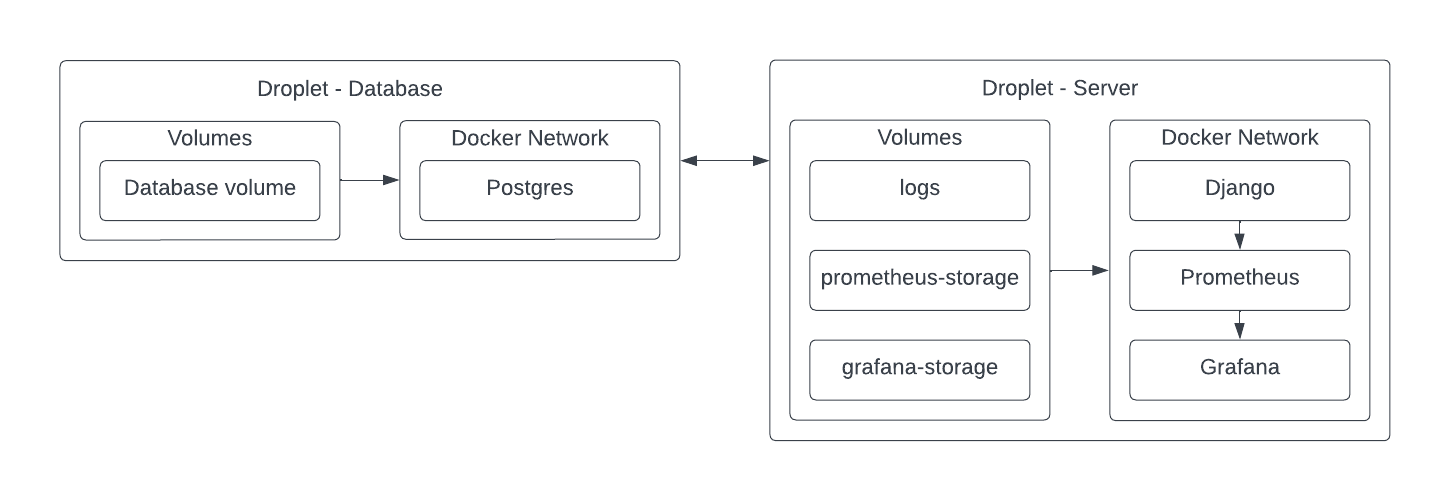
\includegraphics[width=\textwidth]{images/system-architechture.png}
    \caption{Simplified system architecture}
    \label{fig:system-arch}
\end{figure}